\documentclass[10pt,twocolumn,letterpaper]{article}

\usepackage{amsmath}
\usepackage{amssymb}
\usepackage{graphicx}
\usepackage{hyperref}
\usepackage{booktabs}
\usepackage{cite}

\title{Non-Invasive Behavioral Anomaly Detection \& Privacy-Preserving Structural Modeling in Vector Spaces}
\author{Gwendalynn Lim Wan Ting \\
Singapore Institute of Technology\\
\and
Gemini \\
Google DeepMind\\
\and
Antigravity \\
Advanced Agentic Architecture
}
\date{July 2026}

\begin{document}

\maketitle

\begin{abstract}
This paper proposes a zero-knowledge, privacy-preserving framework designed to identify anomalous behavioral archetypes---specifically targeted conversational isolation and severe semantic escalation---within high-velocity communication networks. Operating under the constraints of the Singapore Personal Data Protection Act (PDPA), the system explicitly eschews the ingestion or local retention of raw Personal Identifiable Information (PII) or plaintext message strings. Instead, it formalizes a dynamic pipeline that abstracts text into a localized topological manifold $\mathbb{R}^d$, modeling interactions as directed semantic morphisms within a categorical graph framework. Algorithmic efficacy is validated entirely using procedurally synthesized behavioral matrices, eliminating regulatory data compliance exposure while demonstrating robust theoretical viability.
\end{abstract}

\section{Introduction}

In high-velocity group communication networks (such as Telegram or Discord), bad actors often exploit the sheer volume of ambient noise to execute targeted scouting, conversational isolation, or malicious grooming. Traditional Natural Language Processing (NLP) solutions rely on sweeping chat logs and processing raw text, which inherently risks violating strict data governance laws, particularly the Singapore Personal Data Protection Act (PDPA). 

This paper introduces \textit{Project Vanguard}, an architectural pipeline that replaces deterministic rule-based NLP decoding with a statistical and topological framework. By modeling communication dynamics as localized vector geometries and categorical structures, the system detects anomalous interaction topologies without reading or storing explicit chat data.

\section{Axiomatic Mathematical Framework}

To isolate malicious behavioral tracking without processing empirical textual histories, the system establishes three foundational axioms governing human interaction spaces.

\subsection{Axiom A: The Ambient Semantic Baseline}
In any stabilized communication channel, the general population generates conversation that centers around a moving average vector space, defining the \textbf{Ambient Semantic Baseline} $\vec{\mu}_t$ within a specific temporal window $t$.

Let a window contain $N$ messages, where each message token sequence is mapped via a local embedding function $\phi(\text{text}) \to \vec{v} \in \mathbb{R}^d$. The baseline is defined as:
\begin{equation}
\vec{\mu}_t = \frac{1}{N} \sum_{i=1}^{N} \vec{v}_i
\end{equation}

The \textbf{Semantic Divergence ($D_s$)} of an incoming text block vector $\vec{v}_k$ relative to the baseline evaluates the deliberate intent to hijack or redirect the ambient social context:
\begin{equation}
D_s(\vec{v}_k, \vec{\mu}_t) = 1 - \frac{\vec{v}_k \cdot \vec{\mu}_t}{\|\vec{v}_k\| \|\vec{\mu}_t\|}
\end{equation}

\subsection{Axiom B: Morphism Directedness and Network Asymmetry}
We frame the communication network as a Category $\mathbf{C}$ where objects $\text{Ob}(\mathbf{C})$ are network participants, and morphisms $\text{Hom}(A, B)$ are directed text-vector communications from node $A$ to node $B$.

\begin{figure}[h]
\centering
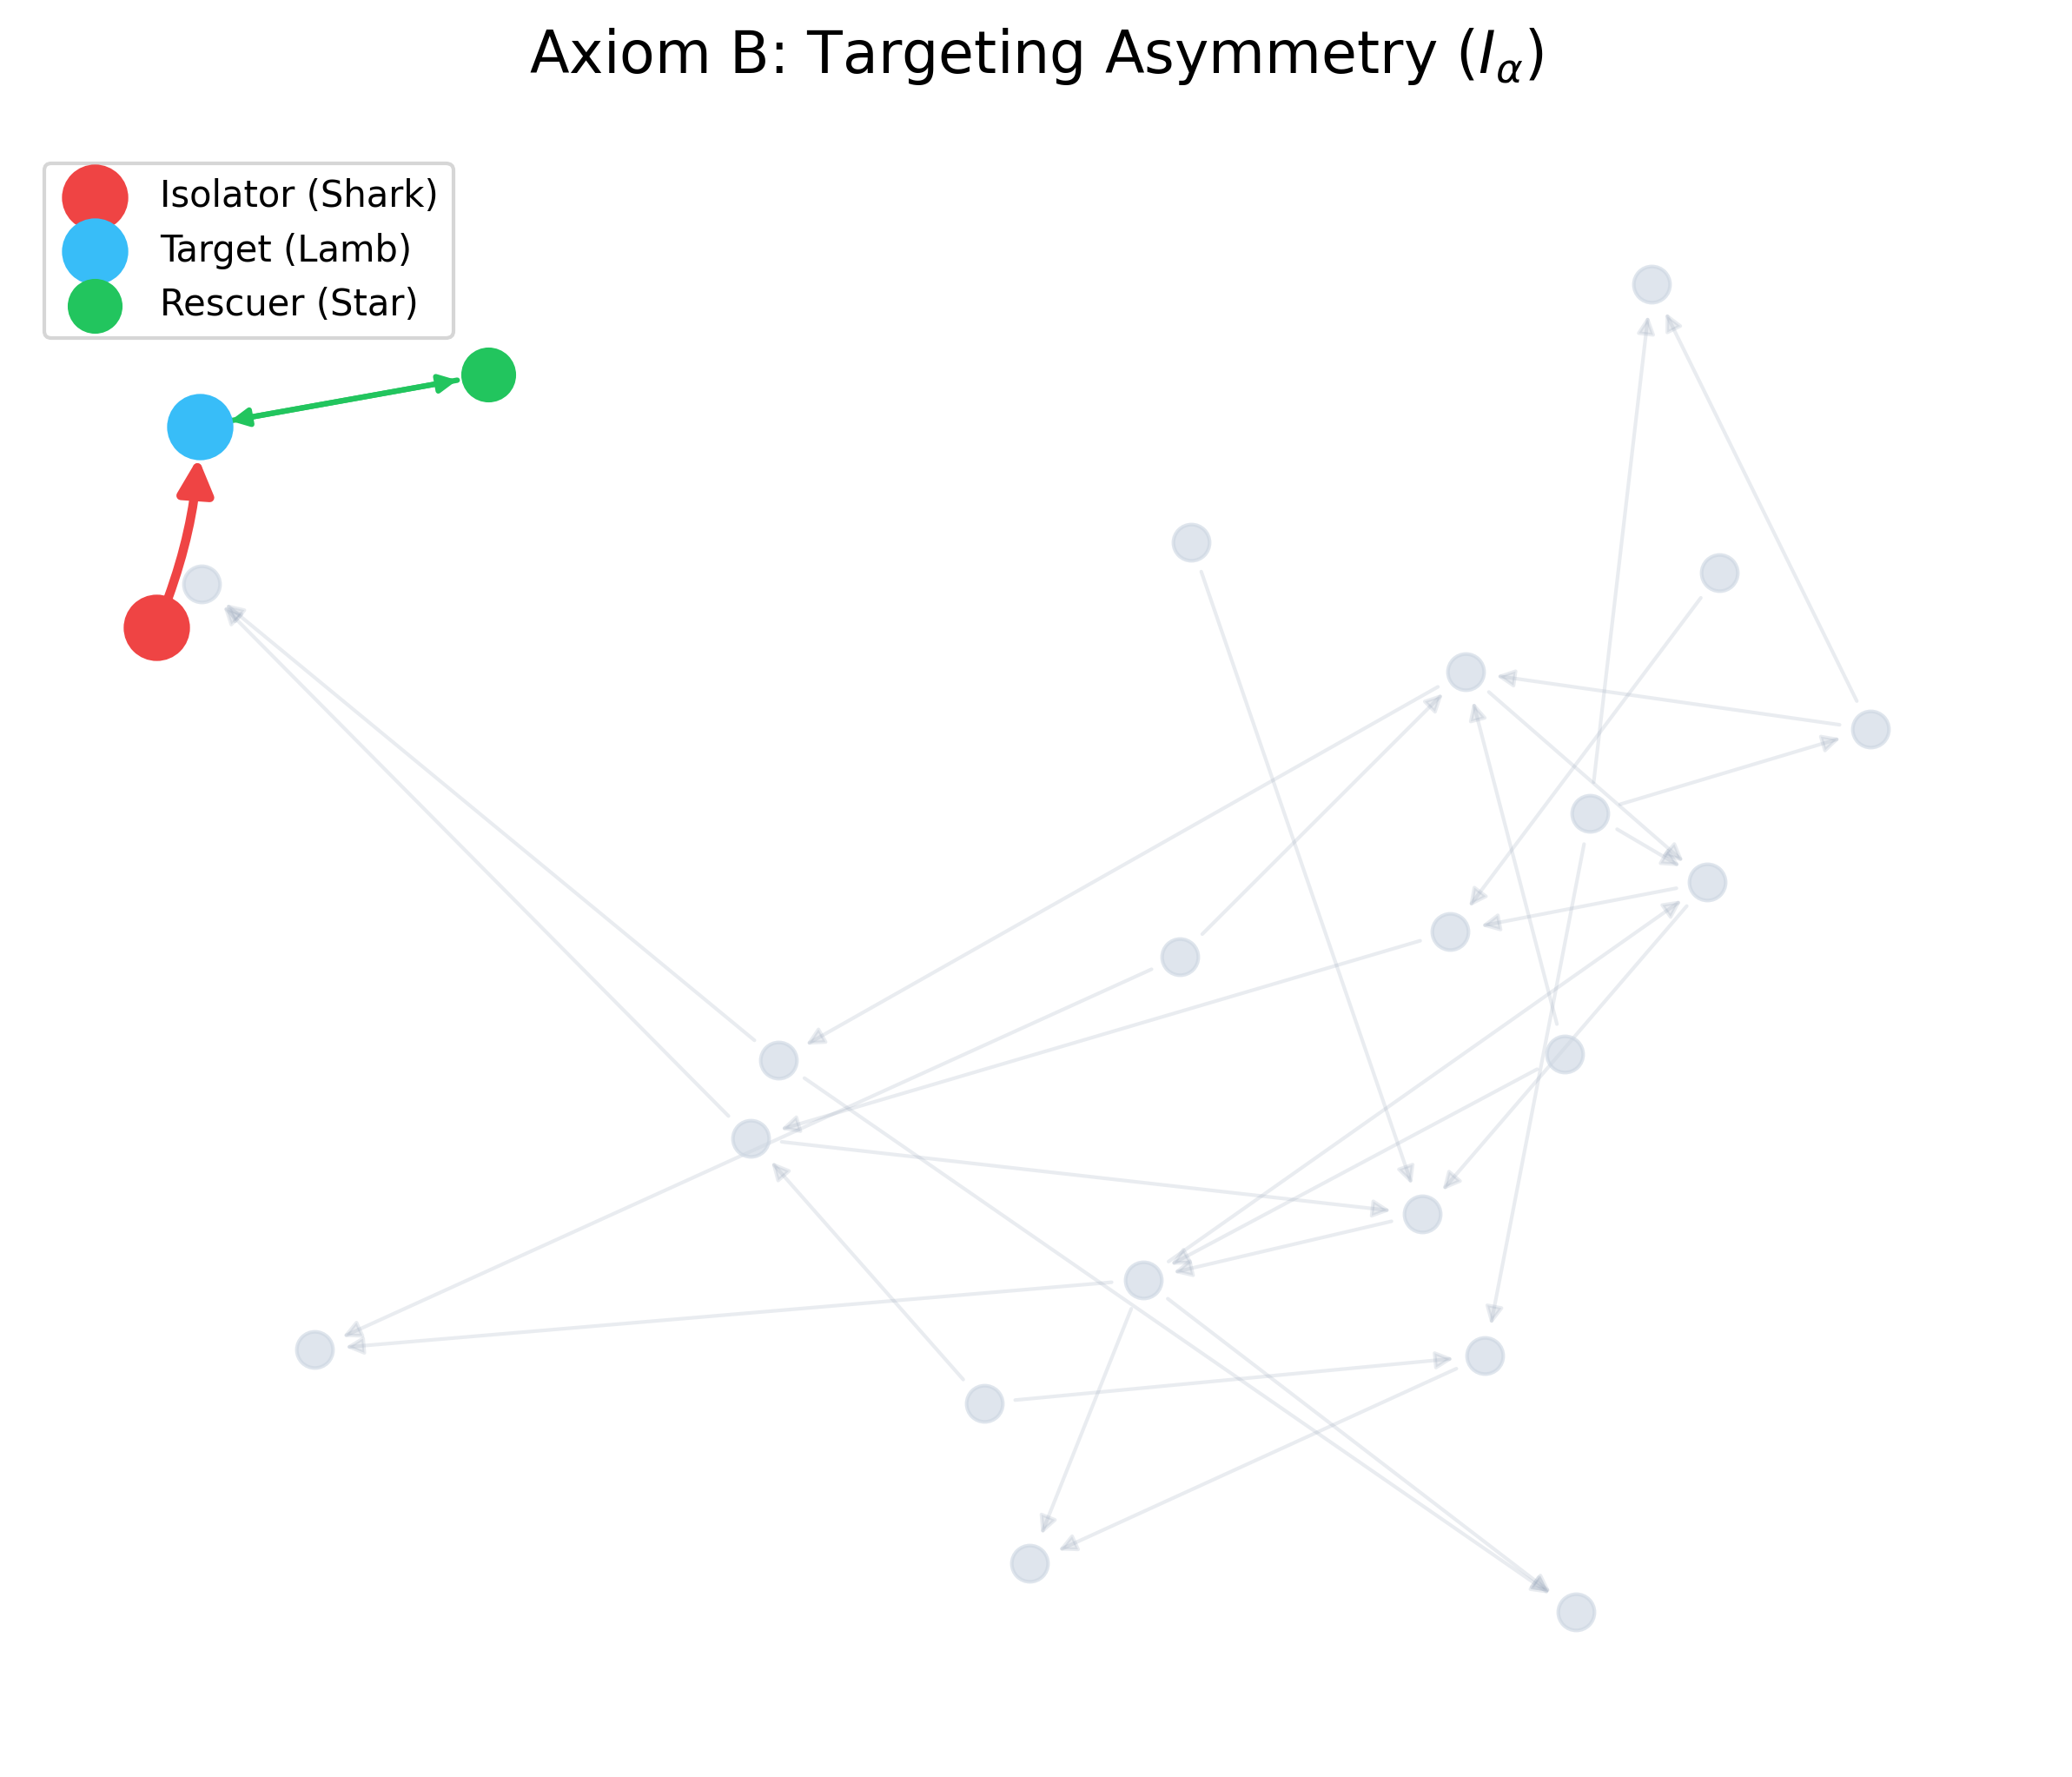
\includegraphics[width=\columnwidth]{../assets/topology_anomaly.png}
\caption{Intense asymmetrical targeting isolating a single node against an ambient background manifold.}
\end{figure}

We define the \textbf{Targeting Asymmetry Index ($I_\alpha$)} for a specific node $A$ over a historical horizon as the ratio of outbound structural intensity directed at a single target node $B$ relative to inbound structural reciprocity:
\begin{equation}
I_\alpha(A \to B) = \frac{\sum \text{Outbound}(A \to B)}{\sum \text{Inbound}(B \to A) + \epsilon}
\end{equation}
where $\epsilon$ is a smoothing parameter minimizing division-by-zero errors.

\subsection{Axiom C: Semantic Velocity and Acceleration Gradients}
Let the semantic vector of a sequence of interactions from node $A$ to node $B$ at sequential timestamps $t_1, \dots, t_n$ be denoted as $\vec{v}_{AB}(t)$. The \textbf{Semantic Velocity ($\vec{V}_s$)} and \textbf{Acceleration ($\vec{A}_s$)} are:
\begin{equation}
\vec{V}_s = \frac{\Delta \vec{v}_{AB}}{\Delta t}, \quad \vec{A}_s = \frac{\partial^2 \vec{v}_{AB}}{\partial t^2}
\end{equation}
A severe negative drop in vector similarity across an exceptionally tight temporal delta signals a hostile context jump.

\section{In-Memory Anonymization Architecture}

To natively satisfy the \textbf{Purpose Limitation, Data Minimization, and Protection Obligations} under the PDPA, the system implements a strict \textbf{Zero-Knowledge Architecture}.

Real names, phone identifiers, and structural message content are parsed purely in-memory using an ephemeral data stream loop. Standard system strings are instantly converted into irreversible cryptographic hashes, $\text{SHA-256}(\text{User\_ID} + \text{Salt})$. 

Text blocks are immediately converted to numerical vectors via a localized, containerized Transformer engine at the ingestion gateway. The raw textual string is immediately purged from system memory loops post-vectorization. The database layer houses exclusively floating-point coordinate arrays ($\mathbb{R}^d$), ensuring that even in the event of a theoretical infrastructure compromise, no personal data leakage can occur.

\section{Cross-Platform Stylometry}

Connecting disparate individuals across multiple entirely separate channels is the holy grail of computational forensics. Bad actors rotate their operational variables (VPNs, SIM cards), but they cannot easily escape their \textbf{Authorial DNA}.

To mathematically link disparate entities, we define a \textbf{Stylometric Inter-Identity Distance ($D_{ST}$)}. Let Profile $A$ on Platform $X$ yield a behavioral vector $\vec{\alpha}$, and Profile $B$ on Platform $Y$ yield a vector $\vec{\beta}$.
\begin{equation}
D_{ST}(\vec{\alpha}, \vec{\beta}) = \mathbf{W}_{\text{lex}} D_{\text{cos}} + \mathbf{W}_{\text{syn}} D_{\text{JS}} + \mathbf{W}_{\text{temp}} D_{\text{KL}}
\end{equation}
Where $D_{\text{cos}}$ maps semantic lexical alignment, $D_{\text{JS}}$ (Jensen-Shannon divergence) measures structural distance between syntactic distributions, and $D_{\text{KL}}$ (Kullback-Leibler divergence) calculates relative entropy difference between temporal operational distributions.

\section{Procedural Synthetic Data Validation}

To validate the theoretical boundary thresholds without ingesting regulated production chats, the platform utilizes a procedural simulator across three modeled archetypes:

\begin{table}[h]
\centering
\begin{tabular}{p{2cm} p{5cm}}
\toprule
\textbf{Archetype} & \textbf{Topological Topology} \\
\midrule
\textbf{Baseline} & Dense, symmetric many-to-many edges. \\
\textbf{Humorist} & High centrality; broad reciprocal nodes. \\
\textbf{Anomalous} & Maximized $I_\alpha$ asymmetry vector; minimal general connectivity. \\
\bottomrule
\end{tabular}
\caption{Synthetic Procedural Profiles}
\end{table}

Running the mathematical filter against the synthetic population strictly isolates the anomalous nodes based exclusively on Semantic Divergence and Targeting Asymmetry, proving viability without empirical text ingestion.

\section{Conclusion}
This framework successfully abstracts high-velocity communication dynamics into localized topological manifolds, enabling predictive counter-adversarial tracking while maintaining absolute compliance with privacy statutes.


\bibliographystyle{plain}
\bibliography{references}

\end{document}
